\documentclass[sigconf]{acmart}
\AtBeginDocument{%
  \providecommand\BibTeX{{%
    \normalfont B\kern-0.5em{\scshape i\kern-0.25em b}\kern-0.8em\TeX}}}
\setcopyright{rightsretained}
\acmConference[QA '22]{Quantum Algorithms Course 2022}{Master CS, Fall 2022}{Leiden, the Netherlands}
\copyrightyear{2022}
\acmYear{2022}
\acmISBN{}
\acmDOI{}
\usepackage[braket, qm]{qcircuit}
\usepackage{subcaption}
%%%% Do not modify lines 1-11

\begin{document}

\title{Research on the Variational Quantum Circuit and Quantum Circuit Partitioning}
\subtitle{Quantum Algorithms --- Course paper} % do not modify thi

\author{Chenyu Shi}
%\orcid{0000-0001-5468-1030}
\email{s3500063@umail.leidenuniv.nl}
\affiliation{
  \institution{LIACS, Leiden University}
  \city{Leiden}
  \country{Netherlands}}

\author{Shupei Li}
%\orcid{0000-0001-5468-1030}
\email{s3430863@umail.leidenuniv.nl}
\affiliation{
  \institution{LIACS, Leiden University}
  \city{Leiden}  
  \country{Netherlands}}

\renewcommand{\shortauthors}{Shi and Li}

\keywords{variational quantum classifier, quantum circuit partitioning, quantum algorithms}

\begin{abstract}
We implement the variational quantum classifier and simulate the large variational quantum circuit with a set of small subcircuits in our project. We evaluate the performance of variational circuits on three open source datasets by performing the five-fold cross validation. Experimental results support the effectiveness of the variational quantum classifier and the validity of the quantum circuit partitioning strategy.
% the abstract summarizes the entire paper: context, problem, solution, approach, data, experimental results, conclusion and real-world implications. but, shortly, so in half a column or so.

\end{abstract}

\maketitle

\section{Introduction}

% textual description of the context, the problem considered, why it is important, how it is addressed in other works, and what real-world applications are. end with a paragraph on what the contributions of the paper are (so, which problems you solve or which research questions you address), and finally a paragraph on how the remainder of the paper is organized.

In this paper, we consider the classification problem from the perspective of quantum algorithms. Classification is an important data analysis task in machine learning field, where a lot of algorithms designed for classical computers have been developed. However, the volume and the variety of data have been growing rapidly in recent several decades. To handle the high-dimensional data with complicated features, we need more advanced techiques and more powerful computers. Developments in quantum computing provide a possible solution for the big data challenge --- introducing quantum algorithms into machine learning to obtain the quantum speedups. In theory, quantum machine learning algorithms outperform classical algorithms by leveraging quantum phenomena (e.g. entanglement and coherence) to reduce the time complexity of information processing and analysis \cite{biamonte2017}. Researchers have successfully designed the quantum version of several machine learning algorithms and implemented them on quantum computers, including both supervised learning and unsupervised learning. For example, Lu and Braunstein proposed the quantum decision tree algorithm based on the quantum fidelity metric \cite{lu2013}. Lloyd et al. performed k-means algorithm with the quantum version of Lloyd’s algorithm \cite{lloyd2013}. There are also attempts to generalize the deep neural networks to quantum computers \cite{qnn2018}. In our project, we focus on using the quantum version of support vector machines (SVMs) to solve the supervised classification problem.

Classical SVMs are widely used in image classification, text mining, etc. The SVM constructs nonlinear decision boundaries by first transforming the feature space and then learning linear boundaries on the transformed space from data. To develop quantum SVMs, we need to map the data into a quantum space and create the corresponding quantum circuits. Havl{\'\i}{\v{c}}ek et al. \cite{havlivcek2019supervised} proposed two strategies to build the quantum SVM model. One strategy is optimizing a variational quantum circuit that is also known as the parametrized quantum circuit. The other is estimating the quantum kernel. Considering the limitations of quantem kernel estimator, we investigate the variational quantum circuit in experiments.

There is a problem in the construction of variational quantum circuits --- the limited number of qubits. Although quantum computers have enormous potential of fast computing, the Noisy Intermediate-Scale Quantum (NISQ) devices suffer from non-negligible noise and limited qubit counts \cite{tang2021}. Therefore, it is meaningful to decompose a large quantum circuit into smaller ones that can be deployed on NISQ devices while maintaining the comparable performance to the original circuit. In the project, we try to simulate the large variational quantum classifier with multiple small quantum circuits. We also explore the generalization ability of our circuit decomposition scheme.

The remainder of the paper is structured as follows. Section 2 reviews previous work related to variational quantum algorithms and quantum circuit cutting. Section 3 explains the variational quantum classifier and quantum circuit cutting strategy in detail. Section 4 introduces datasets we use in the project. We present our experimental set-up and results in Section 5. The paper ends with a conclusion section.

\section{Related work}
% briefly discuss other papers related to this work, or previous work describing other approaches for the same problem. end with a statement on how your paper contributes to these works.

Our project is inspired by the variational quantum algorithms as well as the quantum circuit cutting. We provide an overview on related work in both research directions.

\subsection{Variational Quantum Algorithms}
The variational quantum algorithm is a class of algorithms that imitates traditional methods used on classical computers. Generally, variational quantum algorithms only require a shallow quantum circuit, which can effectively alleviate the impact of noise on NISQ devices and obtain quantum advantages compared to the classical algorithms \cite{cerezo2021}. The core of variational quantum algorithms is an ansatz with a set of trainable parameters. During the training process, data is transformed and fed into the ansatz. And the cost is calculated according to outputs of the ansatz and real labels. The objective of training is minimizing the cost of a pre-defined function.

Variational quantum algorithms have broad application prospects in various fields. In applied mathematics field, Huang et al. \cite{vqa-huang} decompose the transformation matrix into a linear combination of unitaries and optimize the cost function via the variational quantum method. LaRose et al. \cite{vqa-larose} proposed a diagonalization algorithm for principal component analysis, where variational circuit is applied to estimate eigenvalues and eigenvectors. In program compilation field, Khatri et al. \cite{vqa-qc} designed a hybrid algorithm that utilizes the power of both classical and quantum computers to accelerate the compilation of quantum programs. There have also been quantum implementations of machine learning frameworks with variational quantum circuits, such as neural networks for reinforcement learning \cite{vqa-rl}, knowledge graphi \cite{vqa-kg}, etc. In this projetc, we apply the variational quantum circuit as a classifier in supervised learning.

\subsection{Quantum Circuit Partitioning}
To run a large quantum circuit on NISQ devises, we need to partition the large circuit into smaller subcircuits that fit the number of available qubits. Previous studies have investigated several possible schemes of quantum circuit partitioning. \cite{bravyi2016} and \cite{tang2021} both consider a hybrid simulation model. Specially, they access a large circuit by combining the power of classical computers and quantum computers. Some classical postprocessing techniques may be required to reconstruct outputs of the larger quantum circuit. The progess in tensor networks also inspire the development of quantum circuit partition. Peng et al. \cite{peng2020} proposed a time-like circuit cutting strategy that converts a wire in the quantum circuit into the measurement of a qubit and the preparation for the input. Mitarai and Fujii \cite{mitarai2021} presented a space-like partition scheme which decomposes nonlocal gates into a sequence of local operations and simulates the original circuit by sampling. It is worth noting that the size of subcircuits can be further reduced in certain scenarios \cite{marshall2022high}. We try to simulate the variational quantum classifier with smaller circuits in experiments.

\section{Approach}

\subsection{Variational Quantum Classifier}
Variational Quantum Classifier(VQC) is a kind of parameterized quantum circuit used in classification tasks \cite{havlivcek2019supervised}. Conventional machine learning methods, such as SVM and neural networks, often take advantage of a parameterized model as classifiers. During training process, these methods use a target function or loss function to measure the difference between prediction results and ground true labels and update the parameters in the model to improve its performance. After several training epochs on adequate data, these machine learning methods can achieve great performance on prediction on unseen data as well. VQC works in a similar way, whereas applying a quantum circuit as its parameterized model. The abstract model of VQC is shown in Figure \ref{fig:VQC}, including data encoding (or feature mapping) $U_{enc}(x)$, variational model $U_{train}(\theta)$, measurement, and parameter updating(usually via gradient decent). In the following subsection 3.1.1 to 3.1.4, we will introduce these processing steps in detail. And then, in subsection 3.1.5, the overall working principle of our VQC circuit will be discussed.
\begin{figure}[!ht]
	\centering
	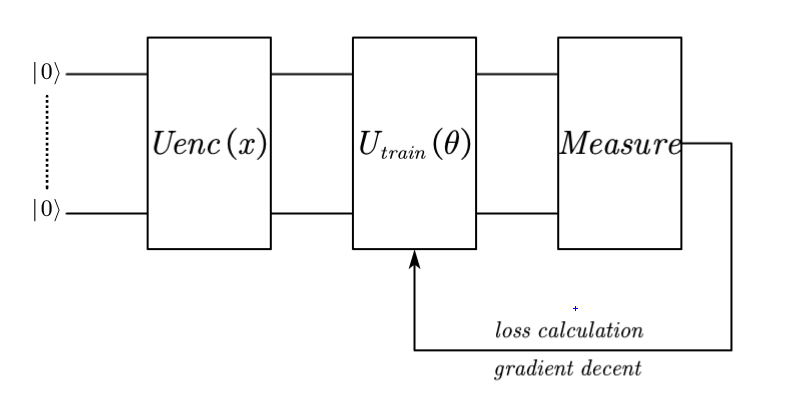
\includegraphics[width=0.48\textwidth]{VQC.png}
	\caption{Abstract model of VQC: {\small \textnormal{ A Variational Quantum Classifier contains these processing steps: data encoding, varational model, measurement and parameter updating.}} }
	\label{fig:VQC}
\end{figure}

\subsubsection{Data Encoding}\hfill\\
As what we have discussed above, VQC attempts to apply parameterized quantum circuit as its learning model. However, nowadays most of data is stored in classical computers which quantum circuit cannot directly access to. Hence, it's necessary to encode classical data into quantum state that can be preocessed by quantum circuit at first. 

There are many basic methods to achieve this encoding preocess, such as basis encoding, amplitude encoding and angle encoding. Besides, several higher order encoding methods which combines different basic encoding methods are studied as well. In this paper, our proposal data encoding method is Pauli feature map, one of the most popular higher order encoding methods. The specific quantum circuit $U_{enc}(x)$ is shown in Figure \ref{fig:encoding} (2-qubit case). As we can see, in this 2-qubit example, the encoding circuit is simplely composed of two Hamdamard gates, three phase gates with the components of the input data $x$ as their parameter and two $CNOT$ gates as the entangling gate. Due to difference of the input data components of each class, the states produced by this circuit will be different as well. In addition, because of the use of entangling gate, the $CNOT$, the state on each qubit will have interaction. Besides, the initial quantum state of each qubit is $\ket{0}$ on account of the requirement of real quantum computers.
\begin{figure}[!ht]
	\centering
	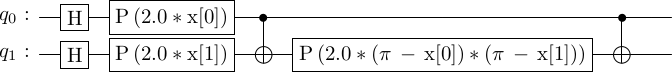
\includegraphics[width=0.48\textwidth]{encode.png}
	\caption{Data encoding circuit: {\small \textnormal{Specific quantum circuit of data encoding in 2-qubit case. This circuit is composed of Hamdamard gates, phase gates, and entangling gate ($CNOT$).}} }
	\label{fig:encoding}
\end{figure}
\subsubsection{Variational Model}\hfill\\
Variational model is a quantum circuit with trainable parameters. During the training process, these parameters will be updated to improve the model's performance. There are various kinds of variational model can be applied in VQC. In this paper, the circuit of our variational model $U_{train}(\theta)$is shown in Figure \ref{fig:variational} (2-qubit case). This 2-qubit example is composed by four y-axis rotation gates parameterized by $\theta$ which is the parameter set to be trained, and one controlled Z gate as the entangling gate. After training, these parameterized rotation gates along with entangling gate can have the ability to convert input states of diverse classes to different output states which can be measured to make a final prediction.   
\begin{figure}[!ht]
	\centering
	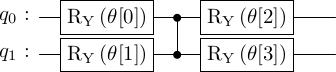
\includegraphics[width=0.48\textwidth]{vari.png}
	\caption{Variational model circuit: {\small \textnormal{Specific quantum circuit of variational model in 2-qubit case. This circuit is composed of parameterized y-axis rotation gates and controlled Z gate.}} }
	\label{fig:variational}
\end{figure}
\subsubsection{Measurement}\hfill\\
 When training most of machine learning models, we need to compare the prediction results and the labels to update parameters, which works the same way in VQC. Nevertheless, after data encoding and variational model, the results are still in quantum states. Hence, we need to extract prediction results from these quantum states. This process is accomplished by measurement. We simply measure all qubits in the circuit and run the circuit for many times. Then we can obtain a distribution of these possible results.
 
 In binary classification tasks, a common way to extract prediction results is to converge the result states distribution into a binary distribution of odd parity states and even parity states. In other words, we consider the parity distribution as the prediction probability of two classes. For example, we run a 2-qubit circuit for 100 times and obtain the measurement result which is [00:21, 01:33, 10:28, 11:18], so the prediction probability for each class shall be [0.39, 0.61]. Therefore, the second class will be predicted as the final result.
\subsubsection{Parameter Updating}\hfill\\
Parameter updating process is the most significant part of machine learning, which includes loss calculation and gradient decent. Loss calculation is the same as the conventional machine learning. When we obtain the predcition probability distribution of each class, we compare the difference between it and ground true label through a loss function. Despite popularity of cross entropy loss in classification tasks, we still choose MAE loss in our model.

In the conventional machine learning, such as neural network, gradient decent based method is famous and efficient to update parameters in the training process. However, it's hard to calculate gradient as in the conventional machine learning due to the fact that our model is based on the quantum circuit. Hence, \cite{schuld2020circuit} proposed a method using difference to subsitute real gradients. In detail, for each parameter $\theta$, we run the circuit and calculate the loss value based on the prediction probability distribution results for parameter $\theta+s$ and $\theta-s$, namely $L(\theta+s)$ and $L(\theta-s)$. Then using the following formula to calculate the gradient:
$$gradient(\theta)=\frac{L(\theta+s)-L(\theta-s)}{2s}$$ 
where $s$ is usually chosen as a small real positive number. Then this proximate gradient is used to update model's parameters just as the same way in the conventional machine learning.

\subsubsection{Overall Analysis}\hfill\\
In this subsection, we make an overal analysis on our VQC and the circuit theoretically to illustrate why this process makes a good classifier.

According to the analysis in the previous subsections, our  ansatz can be written in the mathematical form:
$$U(x,\theta)=U_{train}(\theta)U_{enc}(x)$$

Before the measurement, the following state is prepared:
$$\ket{\psi(x,\theta)}=U(x,\theta)\ket{0^n}$$

And then we measure the observable $Z^{\otimes n}$ on the above state to implement the function:
$$f_\theta(x)=\bra{\psi(x,\theta)}Z^{\otimes n}\ket{\psi(x,\theta)}$$  

This function is actually the expectation of the observing result distribution on the computational basis of even parity states and odd parity states, when giving even parity states value 1 (represent class 0) and odd parity states value -1 (represent class 1). To be more specific, let us use a 2-qubit example to illustrate it.

Suppose we have a general 2-qubit state $\ket{\phi}=a\ket{00}+b\ket{01}+c\ket{10}+d\ket{11}$ as $\ket{\psi(x,\theta)}$. Feed this state into the above function, and the result is actually computed as:
\begin{align*}
	f_\theta(x)&=\bra{\phi}Z^{\otimes n}\ket{\phi}\\
	&=\begin{pmatrix}
		a & b & c & d
		\end{pmatrix}\begin{pmatrix}
		1 & 0 & 0 & 0 \\
		0 & -1 & 0 & 0 \\
		0 & 0 & -1 & 0 \\
		0 & 0 & 0 & 1 
	\end{pmatrix}\begin{pmatrix}
	a \\
	b \\
	c \\
	d 
	\end{pmatrix}\\
    &=a^2-b^2-c^2+d^2
\end{align*}
When we observe $\ket{\phi}$ on the computational basis, the final probability to obtain odd and even parity state shall be:
$$p(even)=p(\ket{00})+p(\ket{11})=a^2+d^2$$
$$p(odd)=p(\ket{01})+p(\ket{10})=b^2+c^2$$

Remember we have given even parity states value 1 and odd parity states value -1 to make it a classifier, so the expectation value of this probability distribution will be:
$$E=1*p(even)+(-1)*p(odd)=a^2-b^2-c^2+d^2$$

It's actually the same result compared to $f_{\theta}(x)$. However, in real cases, we couldn't calculate the exact expectation while adequate repeatation of running the circuit can give us the precise enough approxiamate result. In other words, when we repeat the circuit for enough times, the obtained result distribution can be considered as the real distribution.

Finally, we turn the function $f_{\theta}(x)$ into a (binary) classifier by considering its sign:
$$
h_{\theta}(x)=sign(f_{\theta}(x))=\left\{
\begin{aligned}
	1  & \quad if \ f_{\theta}(x)>0 \\
	-1  & \quad if \ f_{\theta}(x)<0 
\end{aligned}
\right.
$$

Therefore, through adjusting the value of parameter $\theta$ via training process, the input data of different classes will finally have different $h_{\theta}(x)$ function values which makes it an effective classifier.

Finally, our VQC circuit (in 2-qubit case) is shown in Figure \ref{fig:whole}. It combines the  processing steps which have been discussed above. In section 5, we will show and discuss the experimental results of this VQC circuit on different datasets.
\begin{figure*}[!ht]
	\centering
	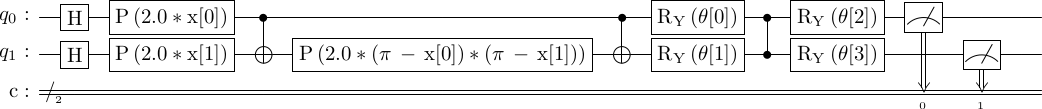
\includegraphics[width=0.9\textwidth]{whole.png}
	\caption{VQC quantum circuit: {\small \textnormal{Our final variational quantum classifier circuit in 2-qubit case. Notice that the initial quantum state of each qubit is always $\ket{0}$.}} }
	\label{fig:whole}
\end{figure*}

\subsection{Quantum Circuit Partitioning}
Quantum circuit partitioning is a technique to evaluate a large quantum circuit only using smaller quantum computers with fewer quantum qubits \cite{marshall2022high}. Many quantum algorithms require more qubits than nowaday quantum computer can really provide, which is a tremendous limitation for designing quantum algorithm. The quantum circuit partition method provides a practical solution to this problem. It divides a larger quantum circuit into several smaller parts which can be run and evaluated individually. Then these results are combined in a polynomial to replicate the output of the larger machine. Various methods of circuit partitioning have been developed to simulate large quantum circuit with fewer qubits, though these methods require more evaluation running times on these divided smaller circuits. In this paper, we mainly apply a method which is proposed in paper \cite{marshall2022high}.

The method in paper \cite{marshall2022high} divides the larger circuit into smaller blocks, and for each block of partition, a new parameterized unitary is added with different parameters $\xi$. Besides, new parameters $\lambda$ are used to combine the observation results of some running of the circuit. In mathematic form of this process can be formulated as:
$$f_{\theta,\xi,\lambda}(x)=\sum_{i\in [L]}\lambda_i\prod_{k\in [K]}\bra{0}U^{k\dagger}(\theta,x,\xi_{i,k})M_kU^k(\theta,x,\xi_{i,k+K})\ket{0}$$

This formula looks rather complicated, but the key point of it can be viewed in Figure \ref{fig:part}. We partition the quantum circuit into two blocks. As we can see, the internal part of each block, $A_{\theta}$ and $B_{\theta}$ remains the same after partitioning. And the operator $G$ which joined two blocks is cut to two parameterized unitary $G_{\xi 1}$ and $G_{\xi 2}$. When simulating the larger circuit, we firstly run each small block individually, and then combine the results by multiplication. Then, each samll block will be operated several times with different initialized learnable parameters $\theta$ and $\xi$ and combine the final results using a weighted sum, where the weights $\lambda$ are also learnable parameters. After training process, the parameters $\lambda$, $\xi$ and $\theta$ can all be updated to simulate the larger circuit and obtain promising results. This method requires running the smaller blocks several more times, which is actually to save space (number of qubits) with time (times of running circuit).

\begin{figure}[!ht]
	\centering
	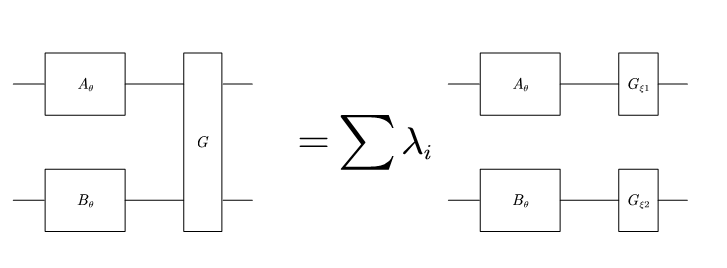
\includegraphics[width=0.45\textwidth]{part.png}
	\caption{Partitioning large circuit: {\small \textnormal{A partitioning method to simulate large quamtum circuit. Notice that new learnable parameters $\lambda$ and $\xi$ are introduced into the smaller circuit block.}} }
	\label{fig:part}
\end{figure}

And one remarkable thing is that we shouldn't initialize the parameters with the same values. Our final result is a weighted sum. For notation simplicity, we write the above formula in this form:
$$f_(x)=\sum \lambda_i g_{\theta i, \xi i}(x).$$
where $g(\cdot)$ represents the multiplication result of each block. Notice that if all parameters are initialized to the same value, the weighted sum becomes meaningless because all $g_{\theta i, \xi i}(x)$ will have same results as well. Besides, the gradients will also be the same, which means this weighted sum actually is equivalent to a single $g(x)$. And it's obviously not the expected result, so we are supposed to initialize the circuits with different parameters and weights.

Finally, our circuits used in experiments are shown in Figure \ref{fig:cutting}, which is an example of cutting 4-qubit circuit into 2-qubit. The experimental results will be show and discussed in Section 5.
\begin{figure*}[!ht]
	\begin{minipage}[t]{0.9\textwidth}%并排放两张图片,每张占页面的0.5,下同。
		\centering
		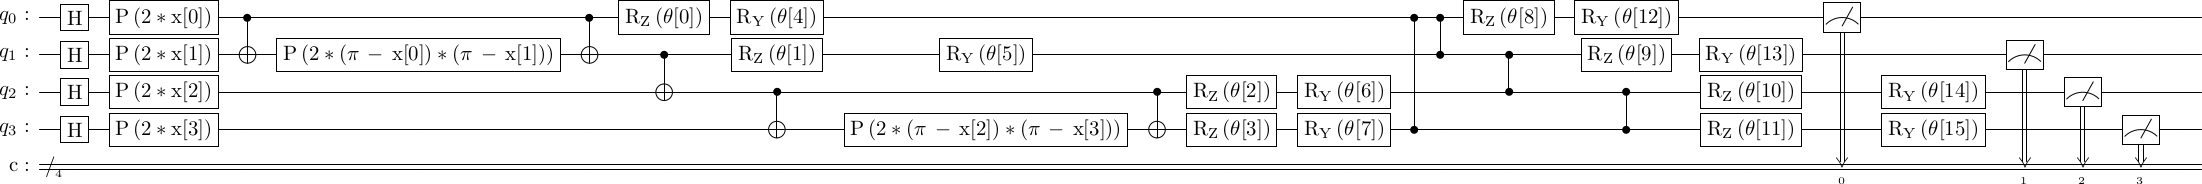
\includegraphics[width=\textwidth]{lar.png}
		\subcaption{Original large circuit} 
	\end{minipage}
	\begin{minipage}[t]{0.9\textwidth}%并排放两张图片,每张占页面的0.5,下同。
		\centering
		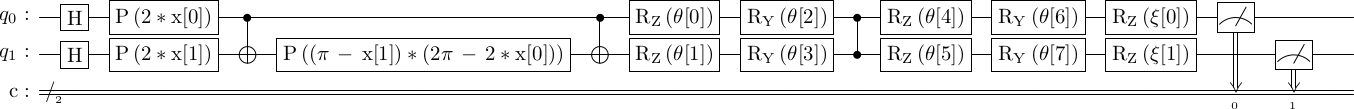
\includegraphics[width=\textwidth]{par1.png}
		\subcaption{Smaller block part 1} 
	\end{minipage}
	\begin{minipage}[t]{0.9\textwidth}%并排放两张图片,每张占页面的0.5,下同。
	    \centering
		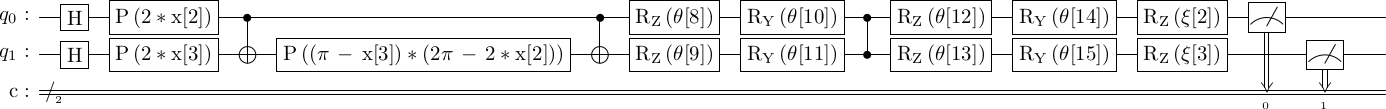
\includegraphics[width=\textwidth]{par2.png}
		\subcaption{Smaller block part 2} 
	\end{minipage}
	\caption{4-qubit to 2-qubit: {\small \textnormal{A partitioning method to simulate large quamtum circuit. Notice that new learnable parameters $\lambda$ and $\xi$ are introduced into the smaller circuit block. To simulate large circuits with smaller one, more running times to evaluate the circuits are required.}} }
	\label{fig:cutting}
\end{figure*}

\section{Data}
We evaluate the variational quantum classifier and the quantum circuit partitioning strategy on three open source datasets: Digits, Moons, and Breast Cancer. We directly use the scikit-learn's built-in version of datasets. The following is a brief overview of data.

\vspace{0.2cm}
\noindent\textbf{Digits}. Digits dataset is a copy of the famous benchmark MNIST in machine learning field. It is composed of handwritten numbers from zero to nine. The original dataset includes 1,797 samples and all ten classes. However, we select a subset of data, whose label is either zero or one, to convert a multi-class classification problem into a binary-class classification problem that fits our quantum circuits. The subset has 320 samples with 64 available features, where the ratio of number zero to number one is 1:1.

\vspace{0.2cm}
\noindent\textbf{Moons}. Moons is a generated dataset in scikit-learn with two features. Its visualization result is two interleaving half circles. The integer label, zero or one, indicates the class membership of each record. We generate 200 samples in experiments. The random state is set to 42 to ensure the reproducibility.

\vspace{0.2cm}
\noindent\textbf{Breast Cancer}. Breast Cancer dataset is a copy of Diagnostic Wisconsin Breast Cancer Data, which is a widely used binary classification dataset. The original data is a set of digitized images that shows a fine needle aspirate of a breast mass. Scikit-learn's version provides the structured data with 30 numeric features calculated from images. These features describe characteristics of cell nuclei, such as radius, symmetry, etc. The number of samples is 569. A malignant tumor belongs to class 0, while a benign one belongs to class 1.

\vspace{0.2cm}
Table \ref{tab:datasets} is a summary of datasets. Note that Moons dataset only has two availble features. Therefore, we use it in the classification task. Digits and Breast Cancer are used both in classification and circuit partitioning.

\begin{table}[!ht]
    \centering
    \caption{Summary of Datasets}
    \label{tab:datasets}
    \begin{tabular}{lllll}
        \toprule
        \textbf{Dataset} & \textbf{\#samples} & \textbf{\#class 0} & \textbf{\#class 1} & \textbf{\#features}\\
        \midrule
        Digits & 320 & 160 & 160 & 64\\
        Moons & 200 & 100 & 100 & 2\\
        Breast Cancer & 569 & 212 & 357 & 30\\
        \bottomrule
    \end{tabular}
\end{table}

% what datasets did you use, what types of networks do they represent, where did you obtain the data? did you do any processing? give a table describing data characteristics, such as number of nodes, edges, average degree, etc.

\section{Experiments}
\subsection{Experimental Setup}
We preprocess features before feeding the data into the quantum circuit. Truncated singular value decomposition technique is appied to reduce dimensionality. Specifically, the number of dimensions of data is reduced to two in classification task, and four in quantum circuit partitioning. We also divide features by the maximum value to scale data. Aiming at assessing the generalization ability of the model, we perform five-fold cross validation in experiments. Average accuracy is calculated according to the performance on five folds and is selected as the metric. Two main hyperparameters in our quantum circuits are \textit{shots} and the learning rate. \textit{shots} is the number of repetitions of the quantum circuit. We set \textit{shots} to 100 in the pilot run and 1,000 in cross validation. The learning rate is optimized via the grid search method. We implement the quantum circuit with Qiskit. Table \ref{tab:software} summarizes the software environment of our experiments.

\begin{table}[!ht]
    \centering
    \caption{Summary of Software Environment}
    \label{tab:software}
    \begin{tabular}{lll}
        \toprule
        \textbf{Item} & \textbf{Version} & \textbf{Function}\\
        \midrule
        Python & 3.9 & Programming language.\\
        Qiskit & 0.22.3 & Quantum circuits.\\
        scikit-learn & 1.2.0 & Datasets and preprocessing.\\
        matplotlib & 3.6.2 & Visualization.\\
        \bottomrule
    \end{tabular}
\end{table}

All experiments are deployed on a local server with an Intel(R) Core(TM) i7-10875H CPU. The source code of our project can be found on GitHub: \url{https://github.com/ShupeiLi/quantum-algorithms-project/tree/master/code}.

\subsection{Results: Variational Quantum Classifier}
Table \ref{tab:vqc-results} reports the experimental results of variational quantum classifier in binary-classification task.

\begin{table}[!ht]
    \centering
    \caption{VQC Results}
    \label{tab:vqc-results}
    \begin{tabular}{lll}
        \toprule
        \textbf{Dataset} & \textbf{Avg. Accuracy} & \textbf{Learning Rate}\\
        \midrule
        Digits & 0.9563 & 0.1\\
        Moons & 0.7850 & 0.01\\
        Breast Cancer & 0.8209 & 0.1\\
        \bottomrule
    \end{tabular}
\end{table}

Figure \ref{fig:contour} shows the visualization of test set in the fourth fold of cross validation. Red triangles represent samples from class 0, while blue triangles are samples from class 1. Contour lines with different colors indicate the decision boundaries of the quantum circuit. We highlight the misclassified samples with yellow circles.

\begin{figure*}[!ht]
    \centering
    \begin{subfigure}{0.45\textwidth}
        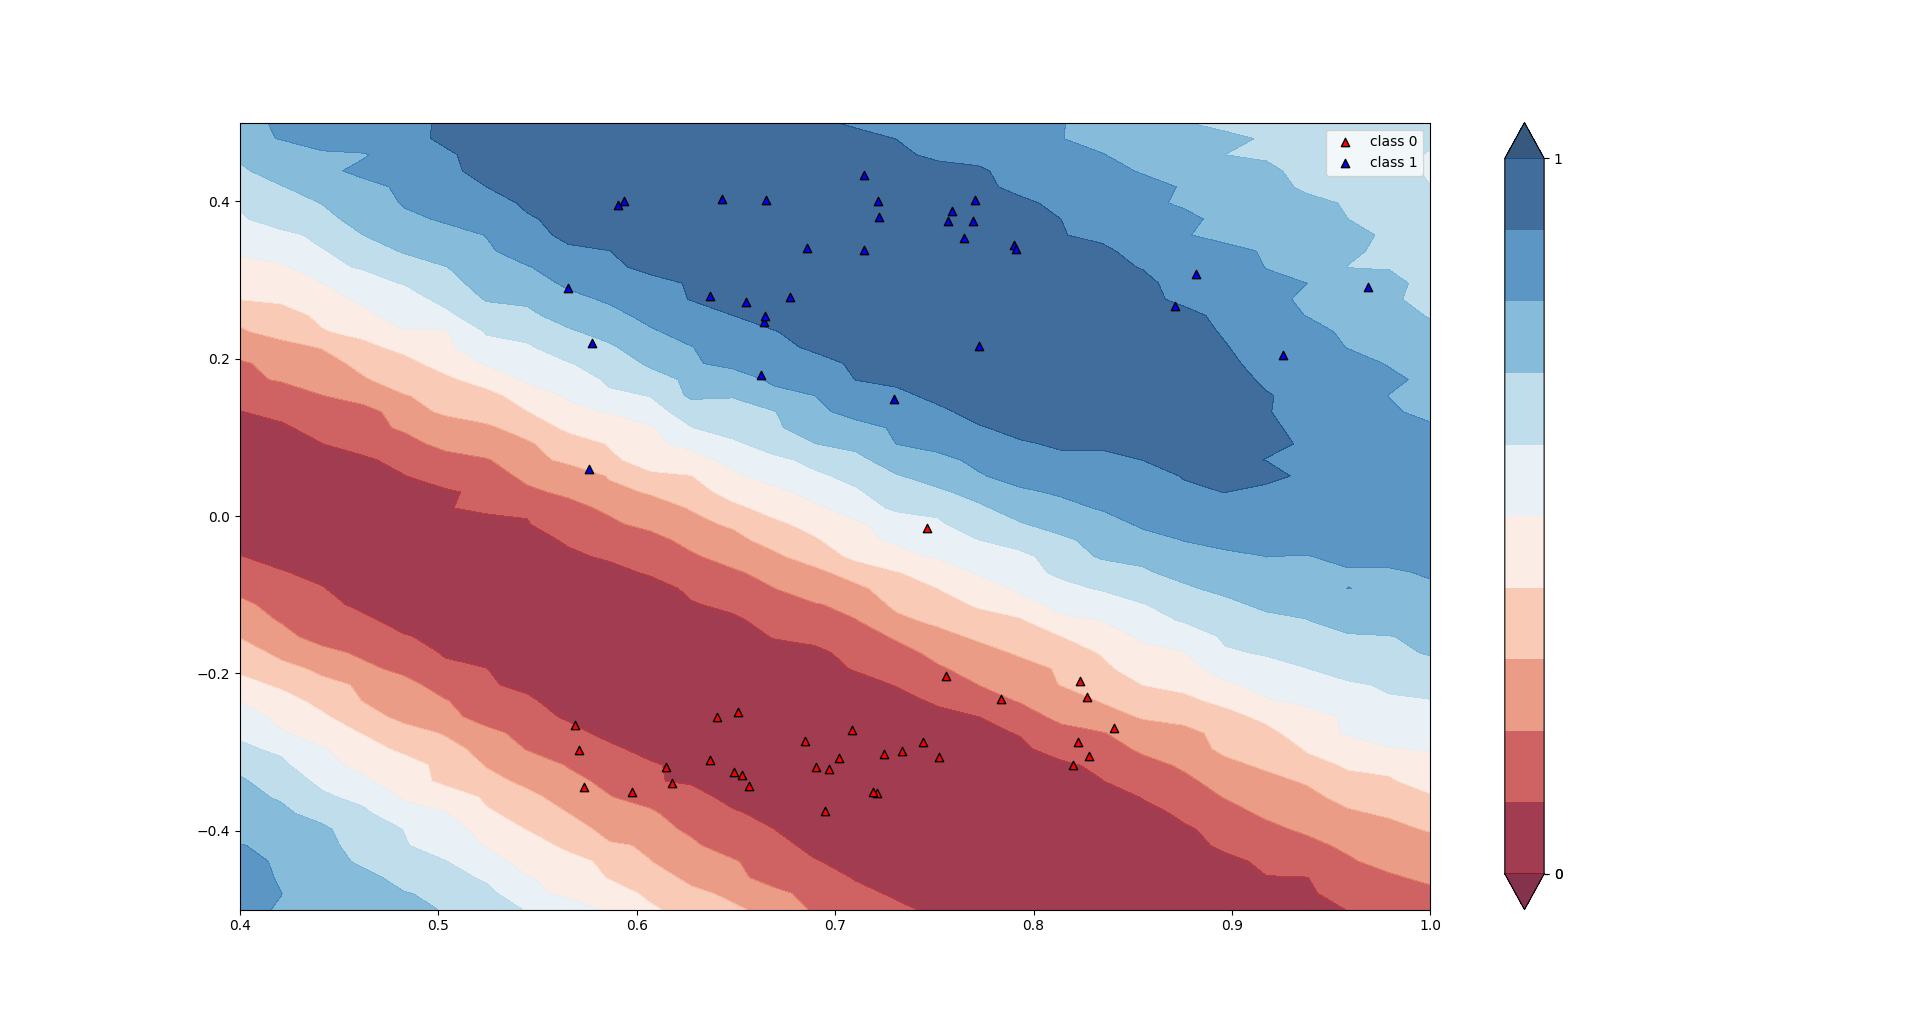
\includegraphics[width=\textwidth]{./digits-2-cv4.png}
        \caption{Contour Plot: Digits}
    \end{subfigure}
    \begin{subfigure}{0.45\textwidth}
        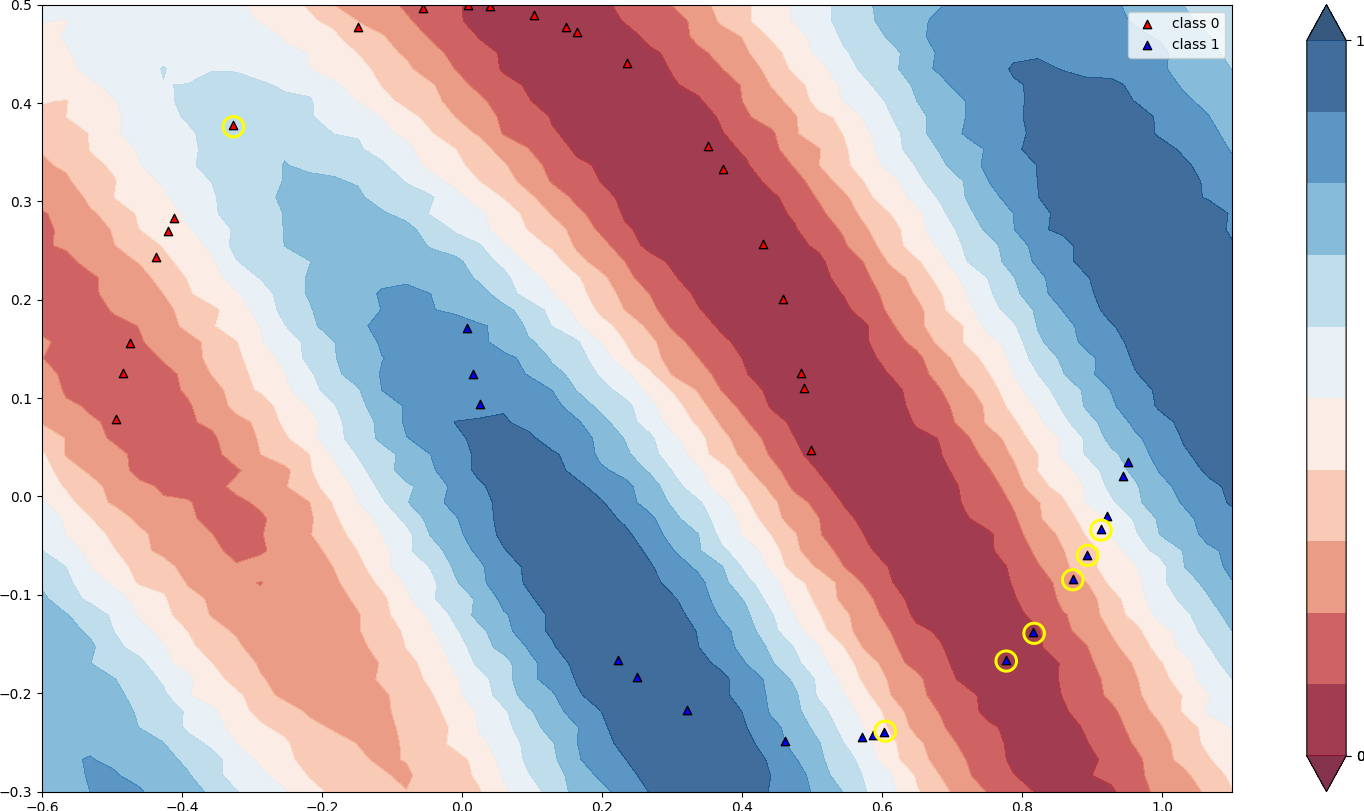
\includegraphics[width=\textwidth]{./moons-cv4.png}
        \caption{Contour Plot: Moons}
    \end{subfigure}
    \begin{subfigure}{0.45\textwidth}
        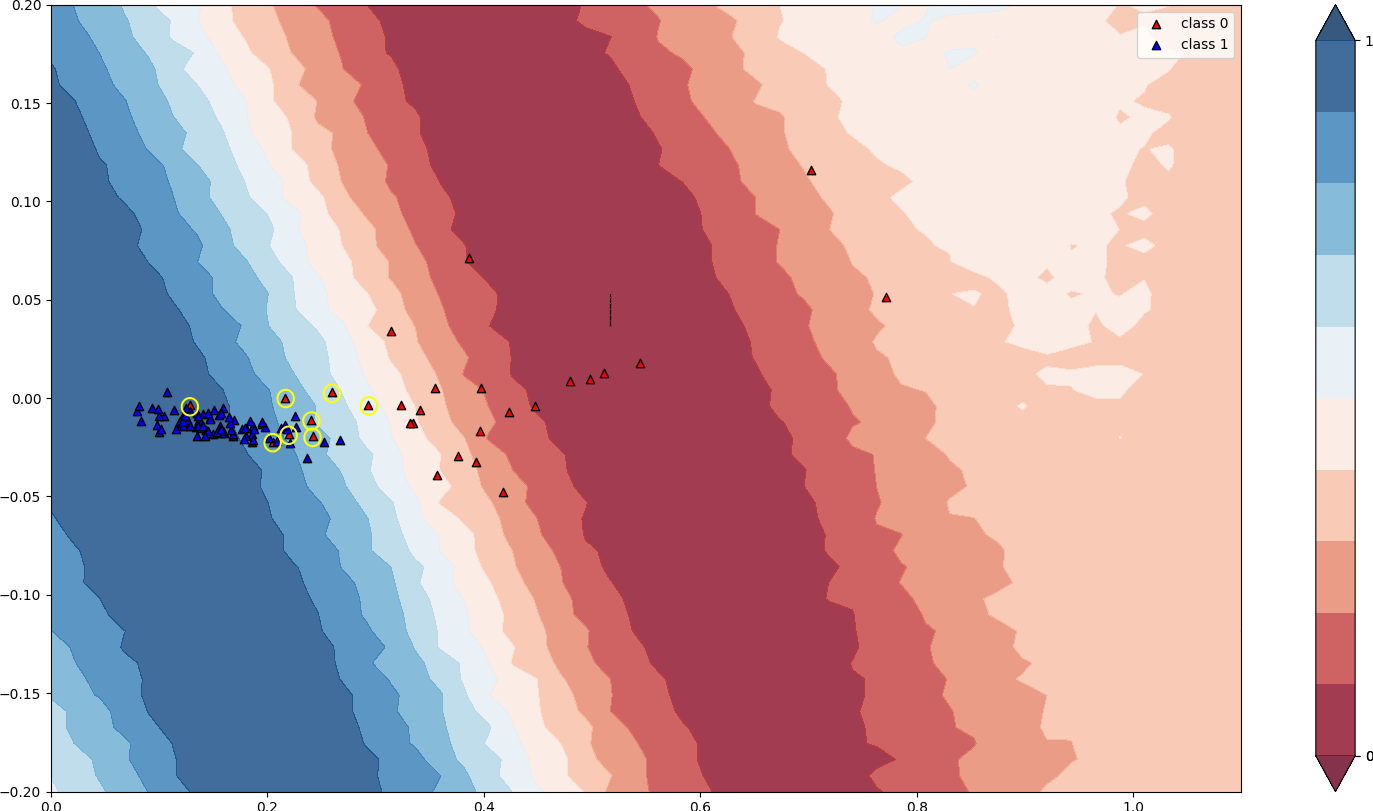
\includegraphics[width=\textwidth]{./cancer-cv4.png}
        \caption{Contour Plot: Breast Cancer}
    \end{subfigure}
    \caption{Visualization of test set in the 4th fold: \textnormal{Draw samples of the test set in contour plots. Red triangles and blue triangles are class 0 and class 1 respectively.}}
    \label{fig:contour}
\end{figure*}

According to Figure \ref{fig:contour}, the variational quantum classifier constructs relatively optimal decision boundaries on Digits dataset, with one misclassified class 0 sample and one misclassified class 1 sample in the fourth fold. However, the variational quantum classifier prefers the false negative error on Moons dataset, while has a bias towards the false positive error on Breast Cancer dataset. The intrinsic bias of classifier may be the cause of the relatively low average accuracy on Moons and Breast Cancer data.

\subsection{Results: Quantum Circuit Partitioning}
In quantum circuit partitioning experiment, we simulate a 4-qubit VQC with only 2-qubit smaller circuits. Table \ref{tab:qcp-results} summarizes the results of quantum circuit partitioning.

\begin{table}[!ht]
    \centering
    \caption{Quantum Circuit Partitioning Results}
    \label{tab:qcp-results}
    \begin{tabular}{llll}
       \toprule 
       \textbf{Dataset} & \textbf{Circuit} & \textbf{Avg. Accuracy} & \textbf{Learning Rate}\\
       \midrule
       Digits & Large circuit & \textbf{0.9688} & 0.1\\
              & Small circuits &  0.9656 & 0.01\\
       Breast & Large circuit & \textbf{0.7612} & 0.01\\
       Cancer & Small circuits & 0.7314 & 0.1\\
       \bottomrule
    \end{tabular}
\end{table}

According to Table \ref{tab:qcp-results}, the large circuit with four qubits performs slghtly better than small subcircuits with two qubits on both datasets. It is consistent with the theory that the set of small subcircuits is an approximation of the original large circuit and is able to achieve the comparable performance. However, the runtime of small circuits is longer than that of the large circuit during the experiment. The reason is that we need to run small circuits with different initialization settings several times to simulate the effect of the large circuit. In our experiment, we call eight small subcircuits to replicate the large circuit. The increase in time complexity is one disadvantage of reducing available qubits. Experimental results support the validity of our quantum circuit partitioning strategy.

% subsections on for example the experimental setup (which software, hardware and parameters did you choose), as well as the results of applying your approach to the data you described in preceding sections, leading to results that answer your research questions. you likely present some tables and figures

\section{Discussion}
In this section, we make a discussion and conclusion of the theoretical analysis and experimental results.

For variational quantum classifier, we could see it works well on most datasets, which means VQC is actually a valid classifer that can be applied to various classification tasks. However, on dataset such as Moons, VQC only has a not bad performance compared to other datasets in the experiment so the performance of VQC can be influenced by the datasets as well. Besides, inputting original data directly often requires large number of qubits in VQC, which is a great limitation to today's quantum computer. Therefore, we have to use external dimensionality reduction or quantum circuit partitioning that has been discussed in the other parts of our experiments.

Quantum circuit partitioning works well in our experiments as well. Smaller circuits with fewer qubits can indeed simulate a large circuit such as VQC well. Additionally, the smaller circuits have a relatively good performance on test sets compared to training sets, which means this partitioning method actually has a generalization ability. Nevertheless, simulating a large circuit with smaller circuits requires more running budget to repeat and evaluate smaller circuits for more times, which is a great limitation of quantum circuit partitioning. 
% summarize in at most one column the main results of the paper, stating how you addressed the problem statement and how the experiments help understand whether  the approach works (or not). end with one or two short suggestions for future work. 

\begin{acks}
% optional: acknowledgments, so people or organizations you wish to thank 
We would like to thank Professor Vedran Dunjko and Course Assistants for the help during the project.
\end{acks}


\bibliographystyle{ACM-Reference-Format}
\bibliography{snacspaper} % put your references in bibtex format in snacspaper.bib

%\appendix
%\section{Robustness checks}
% Appendixes are optional for the course project. they can contain proofs, figures or tables that do not fit in the main body of the text, but are handy as background information

\end{document}
\endinput
